\chapter{Introduction} 
\label{ch:introduction}

% Because of a bug --- Restore original headers:
\fancyhead[ER]{\sffamily\footnotesize{\leftmark}}
\fancyhead[OL]{\sffamily\footnotesize{\rightmark}}

Neoway Business Solution is a Big Data Analytics company with solutions to Sales \& Marketing and Risk \& Compliance that are suited to companies in a variety of business verticals and branches. One of its products is called On Target(OT), a lead recommendation system, based on scoring potential markets according to a given portfolio of clients. The OT will search for leads in a subset of the whole Brazilian's market space, which is composed by all active companies. The user can narrow down the search space based on a set of filters. The Figure \ref{fig:braz-comps-venn-diagram} shows a Venn diagram that illustrates the subsets of the On Target. The \underline{Portfolio} set is composed by the user's clients; The \underline{Market} is where the On Target will search for the leads, it can vary from a set defined by the filters to all the Brazilian active companies (except the user's clients).

\begin{figure}[!ht]
   \centering
   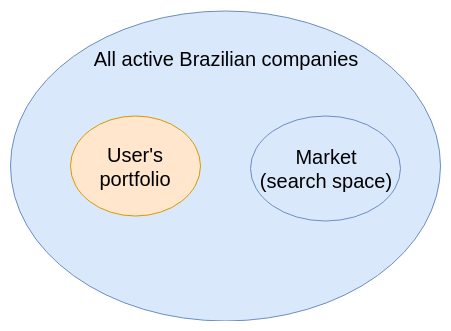
\includegraphics[width=9cm]{fig/ch1-brazil-comps-venn-diagram.png}
   \caption{Venn Diagram representing the sets involved in the recommender system.}
   \label{fig:braz-comps-venn-diagram}
\end{figure}

Recently, the OT was updated, and a benchmark was created to compare between different versions. Overall the new version showed an improvement in the accuracy performance and consistency of the recommendation. By analysing cases in the benchmark, we conjectured that the performance could be further improved in some cases if perhaps the user's portfolio had been pre-clustered before running the recommender system, leading to a more homogeneous and consistent scoring of the market. The last point can be understood through Figure \ref{fig:simi-dist} which shows the distribution of the recommender score in a benchmark case. The recommender system is trained with samples from the user's portfolio and market and its score allows for an interpretation of a similarity measure. The higher the score, going from $0$ to $1$, the more similar is a company to companies in the user's portfolio, i.e. the more similar they are, and are thus better qualified to be converted to a lead or client\footnote{More about the similarity distribution plot will be explained on the chapter \ref{ch:methodology}.}.

\begin{figure}[!ht]
    \begin{subfigure}{\linewidth}
        \centering
        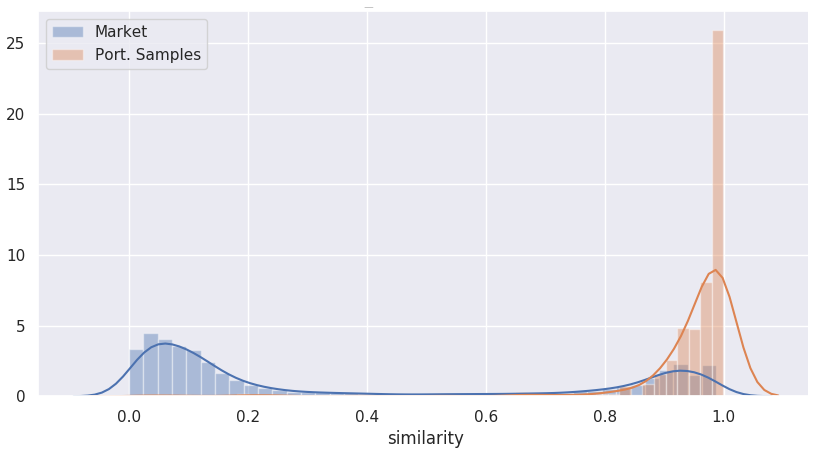
\includegraphics[width=10cm]{fig/ch1-simi-dist-expected.png}
        \caption{}
        \label{fig:simi-dist:expected}
    \end{subfigure}
    \begin{subfigure}{\linewidth}
        \centering
        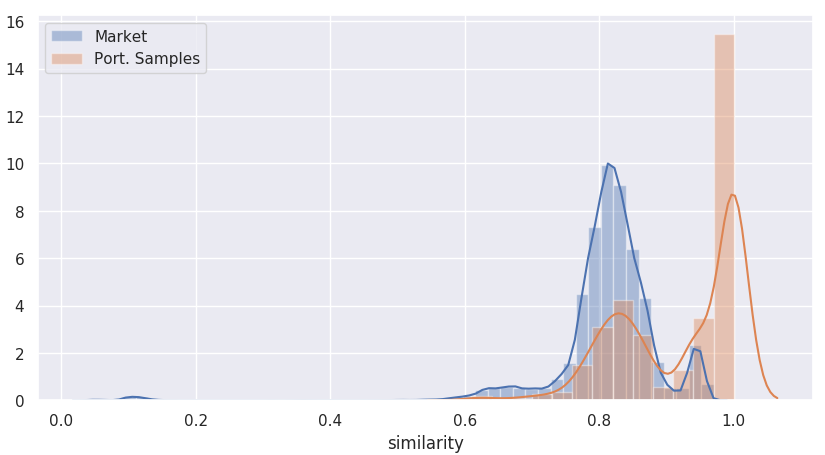
\includegraphics[width=10cm]{fig/ch1-simi-dist-to-investigate.png}
        \caption{}
        \label{fig:simi-dist:to-investigate}
    \end{subfigure}
    \caption{Similarity score from a case at the benchmark. (\subref{fig:simi-dist:expected}) shows a best case scenario one and (\subref{fig:simi-dist:to-investigate}) scenario to be investigated.}
    \label{fig:simi-dist}
\end{figure}

% OBS: "high density probabilities areas" = "bump"
\ref{fig:simi-dist:expected} is the best case scenario of a study, where all the portfolio's samples are close to similarity $1.0$. The market has two high density probabilities areas: one close to similarity $0$ and other close to similarity $1.0$, in others words, some companies have no fit with the portfolio and others are alike the portfolio. The latter is the high quality leads to recommend to the user. \ref{fig:simi-dist:to-investigate} is an example of a study with a behavior that may be improved. The portfolio's sample distribution has two concentrations of mass along the x-axis which can be interpreted that there were two types of customers within the user's portfolio set. The aim of this thesis is to investigate whether this behavior can be improved by a pre-clustering strategy.

One hypothesis of the On Target's team is that in this study (and others alike) the client has a heterogeneous portfolio, \textbf{meaning that it can have two or more distinct profiles in it}. The algorithm tries to optimize for the mean profile of the whole portfolio which may not be the best approach.

This work is one of the several improvements that have been considered in the On Target Product Roadmap. It is a proof of concept which its objective is to analyze whether the overall performance of the high quality leads generation improves by clustering the portfolio before running the recommendation algorithm. 

In order to preserve interpretability, the clustering procedure will not include all available features. Only firmographics data will be used \cite{wikipedia_firmographics} which are data related to characteristics of a business, such as: company size, location, number of employees and others.


\section{Objectives}

\subsection{General Objectives}

The general objective of this work is to analyze whether the performance of the On Target improves by pre-clustering the portfolio with firmographics data before running the recommendation algorithm.

\subsection{Specific Objectives}

Specific objectives of this work are:

\begin{itemize}
    \item defining the pre-clustering strategy;
	\item defining the pre-clustering algorithm;
    \item defining the number of clusters for the benchmark cases;
    \item running On Target against the benchmark with the pre-clustering approach; and
    \item analyzing the distribution of similarity scores and performance metrics against the benchmark.
\end{itemize}


\section{Work outline}

This thesis is organized in the following manner: 

In the Chapter 2 some theoretical concepts are explained, so the reader can understand the what theory is behind this work. 

Next, in the Chapter 3, we introduce the terminology used by the OT's team and a basic view of how it works, later in the chapter, a discussion about the pre-clustering procedures and the conceived experiments.

In Chapter 4, is presented the results of these experiments alongside an extensive analysis in the metrics of several scenarios. 
 
Finally, in Chapter 5, a recap of this work is presented to the reader, with the takeaways. 